\chapter{Herísticas de busca local}

Heurísticas geram soluções viáveis, mas sem garantir a qualidade.

\begin{itemize}
    \item Construtivas
    \item De busca local
\end{itemize}

\section{Introdução}

\subsection{Ótimo local vs. ótimo global}

\begin{center}
    \def\svgwidth{.75\linewidth}
    \import{img/}{otimo_local_global.pdf_tex}
\end{center}

O algoritmo inicia no ponto laranja e vai, incrementalmente, encontrando soluções melhores na vizinhança.

Seguindo o caminho vermelho, ele encontra um mínimo local, já que nenhum vizinho tem um valor de função melhor que ele (menor, já que é um problema de minimização).

Mas seguir o caminho verde, pode ser melhor do que seguir o caminho vermelho.

De qualquer forma, o ótimo global é o roxo, mas a busca local não encontra ele, porque olha apenas a vizinhança.

\textbf{Busca local garante apenas que estamos em um ótimo local, não necessariamente global.}

Também não é possível garantir que o ótimo local é pelo menos próximo do ótimo global. É um ótimo local, mas pode ser ainda muito longe do ótimo global.

Positivo: A solução final é sempre melhor que o ponto de partida.

\subsection{Conceito de vizinhança}

Vizinhança de uma solução é o conjunto de soluções obtidas com uma pequena mudança.

Partindo de uma solução, encontra-se as vizinhas (segundo algum critério). Depois de identificadas as soluções vizinhas, é possível encontrar se existe alguma melhor. Seguindo uma estratégia gulosa, modifica-se a solução inicial partindo para a melhor vizinha.

\begin{example}
    \centering
    \begin{tikzpicture}[every node/.style={fill=white}, n/.style={circle, draw}]
        \node[n, thick, draw=violet] (s) at (0, 0) {19};
        \node[n] (n1) [above right=of s] {11};
        \node[n] (n2) [above left=of s] {25};
        \node[n] (n3) [below left=of s] {14};
        \node[n] (n4) [below right=of s] {50};

        \draw[->, violet] (s) edge (n1);
        \draw (s) edge (n2);
        \draw (s) edge (n3);
        \draw (s) edge (n4);
    \end{tikzpicture}

    \vspace{\baselineskip}

    \begin{tikzpicture}[every node/.style={fill=white}, n/.style={circle, draw}]
        \node[n, thick, draw=violet] (s) at (0, 0) {19};
        \node[n, thick, draw=violet] (n1) [above right=of s] {11};
        \node[n] (n2) [above left=of s] {25};
        \node[n] (n3) [below left=of s] {14};
        \node[n] (n4) [below right=of s] {50};
        \node[n] (n5) [above left=of n1] {27};
        \node[n] (n6) [right=of n1] {7};
        \node[n] (n7) [below right=of n1] {12};

        \draw[->, violet] (s) edge (n1);
        \draw (s) edge (n2);
        \draw (s) edge (n3);
        \draw (s) edge (n4);
        \draw (n1) edge (n5);
        \draw[->, violet] (n1) edge (n6);
        \draw (n1) edge (n7);
    \end{tikzpicture}

    \vspace{\baselineskip}

    \begin{tikzpicture}[every node/.style={fill=white}, n/.style={circle, draw}]
        \node[n, thick, draw=violet] (s) at (0, 0) {19};
        \node[n, thick, draw=violet] (n1) [above right=of s] {11};
        \node[n] (n2) [above left=of s] {25};
        \node[n] (n3) [below left=of s] {14};
        \node[n] (n4) [below right=of s] {50};
        \node[n] (n5) [above left=of n1] {27};
        \node[n, thick, draw=violet] (n6) [right=of n1] {7};
        \node[n] (n7) [below right=of n1] {12};
        \node[n] (n8) [above right=of n6] {17};
        \node[n] (n9) [below right=of n6] {16};

        \draw[->, violet] (s) edge (n1);
        \draw (s) edge (n2);
        \draw (s) edge (n3);
        \draw (s) edge (n4);
        \draw (n1) edge (n5);
        \draw[->, violet] (n1) edge (n6);
        \draw (n1) edge (n7);
        \draw (n6) edge (n8);
        \draw (n6) edge (n9);
    \end{tikzpicture}
\end{example}

Ao final, o nó de valor $7$ é o mínimo local, então é a solução final.

A definição de vizinhança influencia no resultado.

É também importante tomar alguma decisões na hora de percorrer a vizinhança:

\begin{itemize}
    \item First fit - Ao percorrer os vizinhos, quando se encontra um que seja melhor que a solução atual, parte para ele.
    \item Best fit - Verifica \underline{todos} os vizinhos para escolher o melhor: guloso.
    \item Random - Busca aleatória. Mais variedade para encontrar mínimos locais diferentes.
\end{itemize}

Por exemplo, pode ser que depois do nó de valor $14$, exista uma solução melhor ainda.

\begin{example}
    \centering
    \begin{tikzpicture}[every node/.style={fill=white}, n/.style={circle, draw}]
        \node[n, thick, draw=orange] (s) at (0, 0) {19};
        \node[n] (n1) [above right=of s] {11};
        \node[n] (n2) [above left=of s] {25};
        \node[n, thick, draw=orange] (n3) [below left=of s] {14};
        \node[n] (n4) [below right=of s] {50};
        \node[n, thick, draw=orange] (n5) [below right=of n3] {2};

        \draw (s) edge (n1);
        \draw (s) edge (n2);
        \draw[->, orange] (s) edge (n3);
        \draw (s) edge (n4);
        \draw[->, orange] (n3) edge (n5);
    \end{tikzpicture}
\end{example}

First fit normalmente dá passos menores de melhoria, com mais passos. Já o best fit, dá menos passos maiores.

First fit pode ser mais eficiente, mas não necessariamente.

\newpage

\begin{algorithm}
\SetAlgoLined

$S \gets$ Solução inicial\;
\Enqto{Vizinhança da solução atual $S$ tiver uma solução $S'$ melhor}{
    $S \gets S'$\;
}
\Retorna S
\end{algorithm}

A solução inicial pode vir de uma heurística construtiva ou de soluções aleatórias.

Questões: como definir a vizinhança? Como percorrer a vizinhança?

\section{Problema do escalonamento}

\begin{itemize}
    \item \textbf{Entrada:} conjunto de tarefas $\{1, \dots , n\}$, cada tarefa $i$ tem tempo de processamento $t_i$ e $m$ máquinas idênticas.
    \item \textbf{Soluções viáveis:} partição das tarefas em $m$ conjuntos $\left\{ M_1, M_2, \dots , M_m\right\}$.
    \item \textbf{Função objetivo:} $\max\bar{j=1\dots m}\sum_{i \in M_j}t_i$ (makespan).
    \item \textbf{Objetivo:} econtrar solução de custo mínimo.
\end{itemize}

Vizinhança de um escalonamento $\mathcal{M}$: escalonamentos que diferem de $\mathcal{M}$ pela posição de um item.

Seja $l(j) = \sum_{i \in M_j} t_i$ a carga da máquina $j$.

\begin{algorithm}
\SetAlgoLined
\SetKwFunction{EscalonaUm}{EscalonaBuscaLocal}

\Fn{\EscalonaUm{n, t, m}}{
    $\mathcal{M} \gets $ um escalonamento inicial\;
    \tcc{$l(j')$ é o makespan atual}
    \Enqto{houver um item $i'$ na máquina mais carregada $j'$ e uma máquina $j$ tal que $l(j) + t_{i'} < l(j')$}{
        $M_{j'} \gets M_{j'} \setminus \left\{ i'\right\}$\;
        $M_j \gets M_j \cup \left\{ i'\right\}$\;
    }
    \Retorna $\max_{j=1, \dots , m}\sum_{i \in M_j}t_i$
}
\end{algorithm}

\newpage

\begin{example}

    \begin{center}
        $m=2$
    \end{center}

    \begin{multicols}{2}

        \tikzset{tempo/.style 2 args={rectangle split, rectangle split horizontal, draw=#2, rectangle split parts=#1, fill=#2!20}}

        \begin{center}
            \begin{tikzpicture}
                \node[tempo={1}{red}, label=below:$t_1$] (t1) at (0, 0) {};
                \node[tempo={1}{green}, label=below:$t_2$] (t2) [right=of t1] {};
                \node[tempo={2}{blue}, label=below:$t_3$] (t3) [right=of t2] {};
            \end{tikzpicture}
        \end{center}

        \begin{tabular}{l|l}
            $M_1$ & \tikzmark{4m11} \\
            $M_2$ & \tikzmark{4m21} \\
        \end{tabular}

        \begin{tikzpicture}[remember picture, tempo/.append style={anchor=west, overlay}, node distance=1pt]
            \node[tempo={1}{red}] (t1) at (pic cs:4m11) {};
            \node[tempo={1}{green}] (t2) [right=of t1] {};
            \node[tempo={2}{blue}] (t3) [right=of t2] {};
        \end{tikzpicture}

        \begin{center}
            \textit{makespan} = $4$
        \end{center}

        \begin{tabular}{l|l}
            $M_1$ & \tikzmark{5m11} \\
            $M_2$ & \tikzmark{5m21} \\
        \end{tabular}

        \begin{tikzpicture}[remember picture, tempo/.append style={anchor=west, overlay}, node distance=1pt]
            \node[tempo={1}{red}] (t1) at (pic cs:5m11) {};
            \node[tempo={1}{green}] (t2) [right=of t1] {};
            \node[tempo={2}{blue}] (t3) at (pic cs:5m21) {};
        \end{tikzpicture}

        \begin{center}
            \textit{makespan} = $2$
        \end{center}

        \columnbreak

        \begin{center}
            \begin{tikzpicture}
                \node[tempo={1}{red}, label=below:$t_1$] (t1) at (0, 0) {};
                \node[tempo={1}{green}, label=below:$t_2$] (t2) [right=of t1] {};
                \node[tempo={2}{blue}, label=below:$t_3$] (t3) [right=of t2] {};
            \end{tikzpicture}
        \end{center}

        \begin{tabular}{l|l}
            $M_1$ & \tikzmark{4m12} \\
            $M_2$ & \tikzmark{4m22} \\
        \end{tabular}

        \begin{tikzpicture}[remember picture, tempo/.append style={anchor=west, overlay}, node distance=1pt]
            \node[tempo={1}{red}] (t1) at (pic cs:4m12) {};
            \node[tempo={1}{green}] (t2) at (pic cs:4m22) {};
            \node[tempo={2}{blue}] (t3) [right=of t1] {};
        \end{tikzpicture}

        \begin{center}
            \textit{makespan} = $3$
        \end{center}

        \begin{tabular}{l|l}
            $M_1$ & \tikzmark{5m12} \\
            $M_2$ & \tikzmark{5m22} \\
        \end{tabular}

        \begin{tikzpicture}[remember picture, tempo/.append style={anchor=west, overlay}, node distance=1pt]
            \node[tempo={1}{green}] (t2) at (pic cs:5m22) {};
            \node[tempo={1}{red}] (t1) [right=of t2] {};
            \node[tempo={2}{blue}] (t3) at (pic cs:5m12) {};
        \end{tikzpicture}

        \begin{center}
            \textit{makespan} = $2$
        \end{center}
    \end{multicols}
\end{example}

No seguinte exemplo, não há nenhum movimento possível que melhore o resultado.

\begin{example}
    \begin{center}
        $m=2$
    \end{center}

    \tikzset{tempo/.style 2 args={rectangle split, rectangle split horizontal, draw=#2, rectangle split parts=#1, fill=#2!20}}

    \begin{center}
        \begin{tikzpicture}[node distance=.25cm]
            \node[tempo={3}{orange}] (t1) at (0, 0) {};
            \node[tempo={2}{blue}] (t2) [right=of t1] {};
            \node[tempo={2}{red}] (t3) [right=of t2] {};
            \node[tempo={3}{green}] (t4) [right=of t3] {};
            \node[tempo={2}{violet}] (t5) [right=of t4] {};
        \end{tikzpicture}
    \end{center}

    \begin{tabular}{l|l}
        $M_1$ & \tikzmark{6m11} \\
        $M_2$ & \tikzmark{6m21} \\
    \end{tabular}

    \begin{tikzpicture}[remember picture, , tempo/.append style={anchor=west, overlay}, node distance=1pt]
        \node[tempo={3}{orange}] (t1) at (pic cs:6m11) {};
        \node[tempo={3}{green}] (t2) at (pic cs:6m21) {};
        \node[tempo={2}{blue}] (t3) [right=of t1] {};
        \node[tempo={2}{red}] (t4) [right=of t2] {};
        \node[tempo={2}{violet}] (t5) [right=of t3] {};
    \end{tikzpicture}

    \textit{makespan} = $7$
\end{example}

Trocando o conceito de vizinhança para lidar com dois itens de diferença, nós conseguimos encontrar uma solução melhor.

\begin{example}
    \tikzset{tempo/.style 2 args={rectangle split, rectangle split horizontal, draw=#2, rectangle split parts=#1, fill=#2!20}}

    \begin{tabular}{l|l}
        $M_1$ & \tikzmark{7m11} \\
        $M_2$ & \tikzmark{7m21} \\
    \end{tabular}

    \begin{tikzpicture}[remember picture, , tempo/.append style={anchor=west, overlay}, node distance=1pt]
        \node[tempo={2}{red}] (t4) at (pic cs:7m11) {};
        \node[tempo={3}{green}] (t2) at (pic cs:7m21) {};
        \node[tempo={3}{orange}] (t1) [right=of t2] {};
        \node[tempo={2}{blue}] (t3) [right=of t4] {};
        \node[tempo={2}{violet}] (t5) [right=of t3] {};
    \end{tikzpicture}

    \textit{makespan} = $6$
\end{example}

\begin{algorithm}
\SetAlgoLined
\SetKwFunction{EscalonaDois}{EscalonaBuscaLocal2}

\Fn{\EscalonaDois{n, t, m}}{
    $\mathcal{M} \gets$ um escalonamento inicial\;
    \Enqto{houver $i'$ na máquina mais carregada $j'$ e $i$ numa máquina $j$ tal que $l(j) - t_i + t_{i'} < l(j')$ e $l(j') - t_{i'}+t_i<l(j')$}{
        $M_{j'}\gets M_{j'} \setminus \{i'\} \cup \left\{ i\right\}$\;
        $M_j \gets \left\{ i\right\} \cup \left\{ i'\right\}$\;
    }
    \Retorna $\max_{j=1,\dots ,m}\sum_{i \in M_j}t_i$
}
\end{algorithm}

Normalmente as diferentes vizinhanças são combinadas. Iniciando com as vizinhanças mais simples e, quando não dá pra melhorar nada com elas, usa as vizinhanças mais complexas.

\section{Problema do Corte Máximo}

\begin{itemize}
    \item \textbf{Entrada:} um grafo $G = (V, E)$.
    \item \textbf{Soluções viáveis:} um corte de $G$, i.e., um conjunto $S$ tal que $\emptyset\neq S \subset V$.
    \item \textbf{Função objetivo:} número de arestas que sai de $S$, i.e., $|\delta(S)|$.
    \item \textbf{Objetivo:} encontrar solução de custo máximo.
\end{itemize}

Vizinhança de um corte $S$: cortes que tem apenas um vértice a mais ou a menos que $S$.

$c(v) = $ número de arestas incidentes a $v$ que atravessam o corte.

$d(v) = $ número de arestas incidentes a $v$ que não atravessam o corte.

\begin{algorithm}
\SetAlgoLined
\SetKwFunction{CorteUm}{CorteMaximoBuscaLocal}

\Fn{\CorteUm{$G=(V, E)$}}{
    $S \gets $ um corte inicial\;
    $\bar{S} \gets V \setminus S$\;

    \Enqto{houver vértice v tal que $c(v) < d(v)$}{
        \eSe{$v \in S$}{
            $S \gets S \setminus \left\{ v\right\}$\;
            $\bar{S} \gets \bar{S} \cup \left\{ v\right\}$\;
        }{
            $\bar{S} \gets \bar{S} \setminus \left\{ v\right\}$\;
            $S \gets S \cup \left\{ v\right\}$\;
        }
    }
    \Retorna S
}
\end{algorithm}

\begin{example}
    \centering
    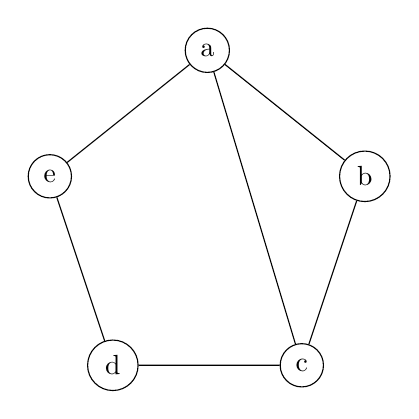
\begin{tikzpicture}[every node/.style={fill=white}, n/.style={circle, draw}, scale=.8]
        \node[n] (a) at (0.5, 2) {a};
        \node[n] (b) at (3, 0) {b};
        \node[n] (c) at (2, -3) {c};
        \node[n] (d) at (-1, -3) {d};
        \node[n] (e) at (-2, 0) {e};

        \draw (a) edge (b);
        \draw (a) edge (c);
        \draw (b) edge (c);
        \draw (c) edge (d);
        \draw (d) edge (e);
        \draw (e) edge (a);
    \end{tikzpicture}

    \vspace{\baselineskip}

    \begin{tikzpicture}[every node/.style={fill=white}, n/.style={circle, draw}]
        \node[n] (a) at (0, 0) {a};
        \node[n] (c) [below=of a] {c};
        \node[n] (e) [below=of c] {e};
        \node[n] (b) at (4, 0) {b};
        \node[n] (d) [below=of b] {d};

        \node[fill=none, draw, ellipse, fit=(a)(c)(e), label=above:$S$] {};
        \node[fill=none, draw, ellipse, fit=(b)(d), label=above:$\bar{S}$] {};

        \draw[thick, red] (a) edge (b);
        \draw (a) edge (c);
        \draw[thick, red] (b) edge (c);
        \draw[thick, red] (c) edge (d);
        \draw[thick, red] (d) edge (e);
        \draw (e) to[out=120, in=-120] (a);
    \end{tikzpicture}

    $c(a) = 1 < 2 = d(a)$

    \vspace{\baselineskip}
    
    \begin{tikzpicture}[every node/.style={fill=white}, n/.style={circle, draw}]
        \node[n] (a) at (4, 0) {a};
        \node[n] (c) at (0, 0) {c};
        \node[n] (e) [below=of c] {e};
        \node[n] (b) [below=of a] {b};
        \node[n] (d) [below=of b] {d};

        \node[fill=none, draw, ellipse, fit=(c)(e), label=above:$S$] {};
        \node[fill=none, draw, ellipse, fit=(a)(b)(d), label=above:$\bar{S}$] {};

        \draw (a) edge (b);
        \draw[thick, red] (a) edge (c);
        \draw[thick, red] (b) edge (c);
        \draw[thick, red] (c) edge (d);
        \draw[thick, red] (d) edge (e);
        \draw[thick, red] (e) edge (a);
    \end{tikzpicture}
\end{example}

Nesse caso, a heurística de busca local melhorou o resultado obtido pelo algoritmo guloso.

\section{Problema da Localicação de Instalações}

Localização de Instalações \underline{sem Capacidades} $\to$ UFL

\begin{itemize}
    \item \textbf{Entrada:} conjunto de clientes $D$, conjunto de instalações $F$, distância $d: D \times F \mapsto \mathbb{R}^+$ e custo de abertura $f: F \mapsto \mathbb{R}^+$.
    \item \textbf{soluções viáveis:} um subconjunto $F'$, tal que $\emptyset \neq F' \subseteq F$.
    \item \textbf{Função objetivo:} custo de abertura mais custo de conexão, i.e., $\sum_{i \in F'} f(i) + \sum_{j \in D}d(j, a(j))$, com $a(j)$ instalação mais próxima de $j$ em $F'$.
    \item \textbf{Objetivo:} encontrar solução de custo mínimo.
\end{itemize}

 Vizinhança de um conjunto de instalações $F'$: conjuntos que tem apenas uma instalação a mais ou a menos que $F'$.

 $D(i) = $ conjunto de clientes mais próximos de $i$ que de qualquer instalação em $F'$. $\to i$ não está em $F'$, mas atrairia esses clientes se estivesse.

 $\Delta(i) = \sum_{j \in D_j}d(j, a(j)) - \sum_{j \in D_i} d(j, i)$. $\to$ Ganho de conexão.

 \begin{algorithm}
 \SetAlgoLined
 \SetKwFunction{UFLUm}{UFL-BuscaLocal}
 \Fn{\UFLUm{D, F, d, f}}{
     $F' \gets $ um conjunto inicial de instalações\;
     \Enqto{houver uma instalação $i'$ tal que $i'\in F'$ com $f(i') > \Delta(i')$ ou $i'\in F \setminus F'$ com $f(i') < \Delta(i')$}{
         \eSe{$i'\in F'$}{
             \tcc{$i'$ não se paga}
             $F' \gets F' \setminus \left\{ i'\right\}$\;
         }{
             \tcc{$i'$ deveria estar aberto}
             $F' \gets F' \cup \left\{ i'\right\}$\;
         }
     }
     \Retorna $F'$
 }
 \end{algorithm}

 \begin{example}
     \includegraphics[width=.8\textwidth]{img/localizacao_instalacoes.png}
 \end{example}

 \section{Problema do caixeiro viajante}

 \begin{itemize}
     \item \textbf{Entrada:} $G = (V, E)$ e função $w$ de peso nas arestas.
     \item \textbf{Soluções viáveis:} circuitos hamiltonianos de $G$.
     \item \textbf{Função objetivo:} soma dos pesos das arestas do circuito.
     \item \textbf{Objetivo:} encontrar um circuito de menor custo.
 \end{itemize}

 Vizinhança 2-OPT de um circuito hamiltoniano $C$: conjunto dos circuitos hamiltonianos que são obtidos trocando 2 arestas de $C$.

 \begin{example}
    \centering
    \begin{multicols}{3}
        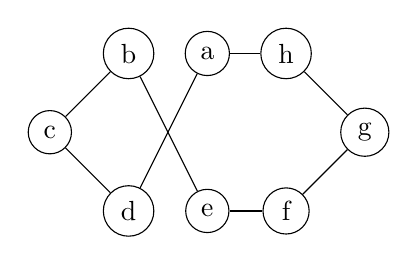
\begin{tikzpicture}[every node/.style={fill=white}, n/.style={circle, draw}]
            \node[n] (c) at (0, 0) {c};
            \node[n] (b) at (1, 1) {b};
            \node[n] (d) at (1, -1) {d};
            \node[n] (a) at (2, 1) {a};
            \node[n] (e) at (2, -1) {e};
            \node[n] (h) at (3, 1) {h};
            \node[n] (f) at (3, -1) {f};
            \node[n] (g) at (4, 0) {g};

            \draw (c) edge (b);
            \draw (b) edge (e);
            \draw (e) edge (f);
            \draw (f) edge (g);
            \draw (g) edge (h);
            \draw (h) edge (a);
            \draw (a) edge (d);
            \draw (d) edge (c);
        \end{tikzpicture}
        \columnbreak
        \vspace*{.8cm}
        {\Huge $\Rightarrow$}
        \columnbreak
        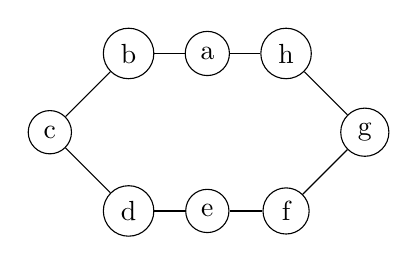
\begin{tikzpicture}[every node/.style={fill=white}, n/.style={circle, draw}]
            \node[n] (c) at (0, 0) {c};
            \node[n] (b) at (1, 1) {b};
            \node[n] (d) at (1, -1) {d};
            \node[n] (a) at (2, 1) {a};
            \node[n] (e) at (2, -1) {e};
            \node[n] (h) at (3, 1) {h};
            \node[n] (f) at (3, -1) {f};
            \node[n] (g) at (4, 0) {g};

            \draw (c) edge (b);
            \draw (b) edge (a);
            \draw (e) edge (f);
            \draw (f) edge (g);
            \draw (g) edge (h);
            \draw (h) edge (a);
            \draw (e) edge (d);
            \draw (d) edge (c);
        \end{tikzpicture}
    \end{multicols}
\end{example}

É importante garantir que a troca permita que a solução seja ainda viável. Por exemplo, a troca a seguir \underline{não} pode ser feita.

\begin{example}
    \centering
    \begin{multicols}{3}
        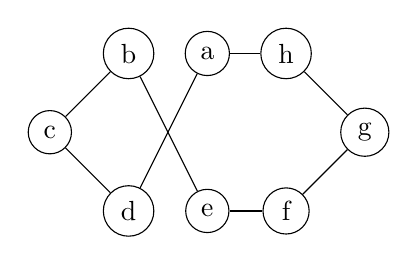
\begin{tikzpicture}[every node/.style={fill=white}, n/.style={circle, draw}]
            \node[n] (c) at (0, 0) {c};
            \node[n] (b) at (1, 1) {b};
            \node[n] (d) at (1, -1) {d};
            \node[n] (a) at (2, 1) {a};
            \node[n] (e) at (2, -1) {e};
            \node[n] (h) at (3, 1) {h};
            \node[n] (f) at (3, -1) {f};
            \node[n] (g) at (4, 0) {g};

            \draw (c) edge (b);
            \draw (b) edge (e);
            \draw (e) edge (f);
            \draw (f) edge (g);
            \draw (g) edge (h);
            \draw (h) edge (a);
            \draw (a) edge (d);
            \draw (d) edge (c);
        \end{tikzpicture}
        \columnbreak
        \vspace*{.8cm}
        {\Huge $\Rightarrow$}
        \columnbreak
        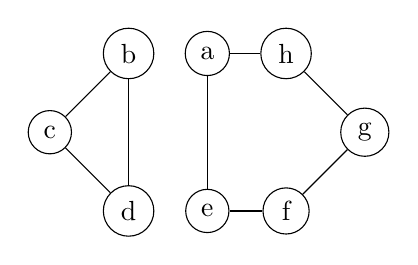
\begin{tikzpicture}[every node/.style={fill=white}, n/.style={circle, draw}]
            \node[n] (c) at (0, 0) {c};
            \node[n] (b) at (1, 1) {b};
            \node[n] (d) at (1, -1) {d};
            \node[n] (a) at (2, 1) {a};
            \node[n] (e) at (2, -1) {e};
            \node[n] (h) at (3, 1) {h};
            \node[n] (f) at (3, -1) {f};
            \node[n] (g) at (4, 0) {g};

            \draw (c) edge (b);
            \draw (e) edge (a);
            \draw (e) edge (f);
            \draw (f) edge (g);
            \draw (g) edge (h);
            \draw (h) edge (a);
            \draw (b) edge (d);
            \draw (d) edge (c);
        \end{tikzpicture}
    \end{multicols}
\end{example}

\begin{algorithm}
\SetAlgoLined
\SetKwFunction{TSPCinco}{TSP-2-OPT}
\Fn{\TSPCinco{$G=(V, E), w$}}{
    $C \gets$ um circuito hamiltoniano inicial\;
    \Enqto{houver um par de arestas $(u, v)$ e $(x, z)$ em $C$ tal que $w(u, x) + w(x, z) < w(u, v) + w(x, z)$}{
        $C \gets C \setminus \left\{ (u, v), (x, z)\right\} \cup \left\{ (u, x), (v, z)\right\}$\;
    }
    \Retorna C
}
\end{algorithm}

É possível utilizar uma vizinhança 3-OPT.

\begin{example}
    \centering
    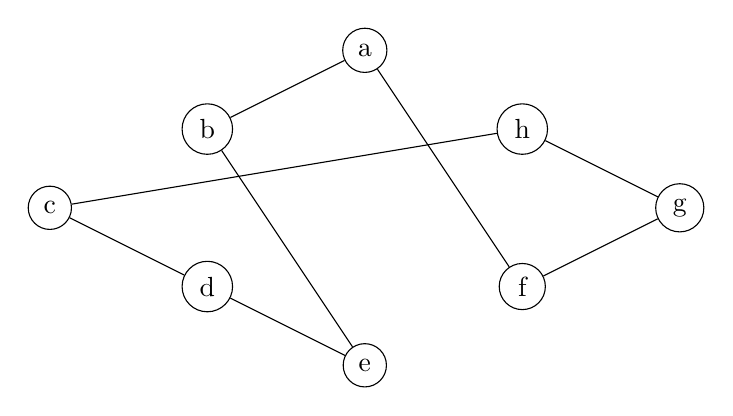
\begin{tikzpicture}[every node/.style={fill=white}, n/.style={circle, draw}]
        \node[n] (a) at (0, 0) {a};
        \node[n] (b) at (-2, -1) {b};
        \node[n] (c) at (-4, -2) {c};
        \node[n] (d) at (-2, -3) {d};
        \node[n] (e) at (0, -4) {e};
        \node[n] (f) at (2, -3) {f};
        \node[n] (g) at (4, -2) {g};
        \node[n] (h) at (2, -1) {h};

        \draw (a) edge (b);
        \draw (b) edge (e);
        \draw (e) edge (d);
        \draw (d) edge (c);
        \draw (c) edge (h);
        \draw (h) edge (g);
        \draw (g) edge (f);
        \draw (f) edge (a);
    \end{tikzpicture}

    \vspace{\baselineskip}
    
    {\Huge $\Downarrow$}
    
    \vspace{\baselineskip}
    
    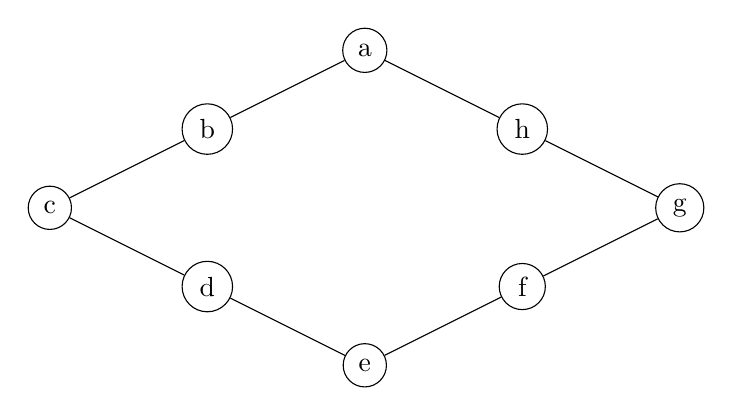
\begin{tikzpicture}[every node/.style={fill=white}, n/.style={circle, draw}]
        \node[n] (a) at (0, 0) {a};
        \node[n] (b) at (-2, -1) {b};
        \node[n] (c) at (-4, -2) {c};
        \node[n] (d) at (-2, -3) {d};
        \node[n] (e) at (0, -4) {e};
        \node[n] (f) at (2, -3) {f};
        \node[n] (g) at (4, -2) {g};
        \node[n] (h) at (2, -1) {h};

        \draw (a) edge (b);
        \draw (b) edge (c);
        \draw (c) edge (d);
        \draw (d) edge (e);
        \draw (e) edge (f);
        \draw (f) edge (g);
        \draw (g) edge (h);
        \draw (h) edge (a);
    \end{tikzpicture}
\end{example}

Na realidade é possível usar uma vizinhança k-OPT mais geral. Uma \textbf{categoria de vizinhanças}.

\section{Metaheurísticas de busca}

Extensões da busca local. Como fugir do mínimo local?

\begin{itemize}
    \item Repeated local search
    \item Simulated annealing
    \item Tabu search
    \item Variable neighbourhood search
    \item GRASP
\end{itemize}

\subsection{Repeated local search}

Realizar diversas buscas locais com instâncias e buscas aleatórias. Joga diferentes pontos iniciais de busca, para que alguma delas encontre uma solução razoável.

\begin{center}
    \def\svgwidth{.75\linewidth}
    \import{img/}{repeated_local_search.pdf_tex}
\end{center}

\newpage

\subsection{Simulated annealing (Cozimento simulado)}

Ideia de temperatura. Enquanto a temperatura do sistema está alta, a busca tem grande chance de fazer escolhas que piorem a solução.

O algoritmo busca o espaço ao redor da solução inicial de forma mais aleatória (podendo ir para soluções piores), mas conforme o tempo passa (temperatura abaixa), converge para um mínimo local.

\begin{center}
    \def\svgwidth{.75\linewidth}
    \import{img/}{simulated_annealing.pdf_tex}
\end{center}

\subsection{Tabu seach}

No início faz uma busca local até um mínimo local. Chegando no mínimo, ele passa a aceitar vizinhos que piorem para escapar do mínimo local. Espera encontrar em algum ponto um mínimo local melhor que o anterior.

\begin{center}
    \def\svgwidth{.75\linewidth}
    \import{img/}{tabu_search.pdf_tex}
\end{center}

Existe uma questão que, enquanto ``sobe o morro'', sempre há pelo menos uma solução melhor (a que você veio antes). Para isso, tem que ter uma lista tabu indicando que soluções já percorreu e proibir essses movimentos.

\subsection{Variable neighbourhood search}

Usa uma vizinhança mais simples. Quando chega em um mínimo local, usa uma vizinhança mais complexa e depois volta para a vizinhança mais simples. Pode usar diversos níveis de complexidade de vizinhanças.

\subsection{GRASP - Greed Randomized Adaptive Search Procedure}

Combina estratégia gulosa com aleatoriedade e busca local. Aleatoriza os algoritmos gulosos para que cada vez que executa, ele percorra um caminho diferente trazendo diversidade de soluções. Em cada passo, tem também um processo de busca local para melhorar o resultado obtido pelo algoritmo guloso.
